\batchmode
\documentclass[10pt,notoc]{cekarticle}
\RequirePackage{ifthen}


\usepackage{array}
\usepackage{wrapfig}


\usepackage[dvips]{color}


\pagecolor[gray]{.7}

\usepackage[]{inputenc}



\makeatletter

\makeatletter
\count@=\the\catcode`\_ \catcode`\_=8 
\newenvironment{tex2html_wrap}{}{}%
\catcode`\<=12\catcode`\_=\count@
\newcommand{\providedcommand}[1]{\expandafter\providecommand\csname #1\endcsname}%
\newcommand{\renewedcommand}[1]{\expandafter\providecommand\csname #1\endcsname{}%
  \expandafter\renewcommand\csname #1\endcsname}%
\newcommand{\newedenvironment}[1]{\newenvironment{#1}{}{}\renewenvironment{#1}}%
\let\newedcommand\renewedcommand
\let\renewedenvironment\newedenvironment
\makeatother
\let\mathon=$
\let\mathoff=$
\ifx\AtBeginDocument\undefined \newcommand{\AtBeginDocument}[1]{}\fi
\newbox\sizebox
\setlength{\hoffset}{0pt}\setlength{\voffset}{0pt}
\addtolength{\textheight}{\footskip}\setlength{\footskip}{0pt}
\addtolength{\textheight}{\topmargin}\setlength{\topmargin}{0pt}
\addtolength{\textheight}{\headheight}\setlength{\headheight}{0pt}
\addtolength{\textheight}{\headsep}\setlength{\headsep}{0pt}
\setlength{\textwidth}{349pt}
\newwrite\lthtmlwrite
\makeatletter
\let\realnormalsize=\normalsize
\global\topskip=2sp
\def\preveqno{}\let\real@float=\@float \let\realend@float=\end@float
\def\@float{\let\@savefreelist\@freelist\real@float}
\def\liih@math{\ifmmode$\else\bad@math\fi}
\def\end@float{\realend@float\global\let\@freelist\@savefreelist}
\let\real@dbflt=\@dbflt \let\end@dblfloat=\end@float
\let\@largefloatcheck=\relax
\let\if@boxedmulticols=\iftrue
\def\@dbflt{\let\@savefreelist\@freelist\real@dbflt}
\def\adjustnormalsize{\def\normalsize{\mathsurround=0pt \realnormalsize
 \parindent=0pt\abovedisplayskip=0pt\belowdisplayskip=0pt}%
 \def\phantompar{\csname par\endcsname}\normalsize}%
\def\lthtmltypeout#1{{\let\protect\string \immediate\write\lthtmlwrite{#1}}}%
\newcommand\lthtmlhboxmathA{\adjustnormalsize\setbox\sizebox=\hbox\bgroup\kern.05em }%
\newcommand\lthtmlhboxmathB{\adjustnormalsize\setbox\sizebox=\hbox to\hsize\bgroup\hfill }%
\newcommand\lthtmlvboxmathA{\adjustnormalsize\setbox\sizebox=\vbox\bgroup %
 \let\ifinner=\iffalse \let\)\liih@math }%
\newcommand\lthtmlboxmathZ{\@next\next\@currlist{}{\def\next{\voidb@x}}%
 \expandafter\box\next\egroup}%
\newcommand\lthtmlmathtype[1]{\gdef\lthtmlmathenv{#1}}%
\newcommand\lthtmllogmath{\lthtmltypeout{l2hSize %
:\lthtmlmathenv:\the\ht\sizebox::\the\dp\sizebox::\the\wd\sizebox.\preveqno}}%
\newcommand\lthtmlfigureA[1]{\let\@savefreelist\@freelist
       \lthtmlmathtype{#1}\lthtmlvboxmathA}%
\newcommand\lthtmlpictureA{\bgroup\catcode`\_=8 \lthtmlpictureB}%
\newcommand\lthtmlpictureB[1]{\lthtmlmathtype{#1}\egroup
       \let\@savefreelist\@freelist \lthtmlhboxmathB}%
\newcommand\lthtmlpictureZ[1]{\hfill\lthtmlfigureZ}%
\newcommand\lthtmlfigureZ{\lthtmlboxmathZ\lthtmllogmath\copy\sizebox
       \global\let\@freelist\@savefreelist}%
\newcommand\lthtmldisplayA{\bgroup\catcode`\_=8 \lthtmldisplayAi}%
\newcommand\lthtmldisplayAi[1]{\lthtmlmathtype{#1}\egroup\lthtmlvboxmathA}%
\newcommand\lthtmldisplayB[1]{\edef\preveqno{(\theequation)}%
  \lthtmldisplayA{#1}\let\@eqnnum\relax}%
\newcommand\lthtmldisplayZ{\lthtmlboxmathZ\lthtmllogmath\lthtmlsetmath}%
\newcommand\lthtmlinlinemathA{\bgroup\catcode`\_=8 \lthtmlinlinemathB}
\newcommand\lthtmlinlinemathB[1]{\lthtmlmathtype{#1}\egroup\lthtmlhboxmathA
  \vrule height1.5ex width0pt }%
\newcommand\lthtmlinlineA{\bgroup\catcode`\_=8 \lthtmlinlineB}%
\newcommand\lthtmlinlineB[1]{\lthtmlmathtype{#1}\egroup\lthtmlhboxmathA}%
\newcommand\lthtmlinlineZ{\egroup\expandafter\ifdim\dp\sizebox>0pt %
  \expandafter\centerinlinemath\fi\lthtmllogmath\lthtmlsetinline}
\newcommand\lthtmlinlinemathZ{\egroup\expandafter\ifdim\dp\sizebox>0pt %
  \expandafter\centerinlinemath\fi\lthtmllogmath\lthtmlsetmath}
\newcommand\lthtmlindisplaymathZ{\egroup %
  \centerinlinemath\lthtmllogmath\lthtmlsetmath}
\def\lthtmlsetinline{\hbox{\vrule width.1em \vtop{\vbox{%
  \kern.1em\copy\sizebox}\ifdim\dp\sizebox>0pt\kern.1em\else\kern.3pt\fi
  \ifdim\hsize>\wd\sizebox \hrule depth1pt\fi}}}
\def\lthtmlsetmath{\hbox{\vrule width.1em\kern-.05em\vtop{\vbox{%
  \kern.1em\kern0.8 pt\hbox{\hglue.17em\copy\sizebox\hglue0.8 pt}}\kern.3pt%
  \ifdim\dp\sizebox>0pt\kern.1em\fi \kern0.8 pt%
  \ifdim\hsize>\wd\sizebox \hrule depth1pt\fi}}}
\def\centerinlinemath{%
  \dimen1=\ifdim\ht\sizebox<\dp\sizebox \dp\sizebox\else\ht\sizebox\fi
  \advance\dimen1by.5pt \vrule width0pt height\dimen1 depth\dimen1 
 \dp\sizebox=\dimen1\ht\sizebox=\dimen1\relax}

\def\lthtmlcheckvsize{\ifdim\ht\sizebox<\vsize 
  \ifdim\wd\sizebox<\hsize\expandafter\hfill\fi \expandafter\vfill
  \else\expandafter\vss\fi}%
\providecommand{\selectlanguage}[1]{}%
\makeatletter \tracingstats = 1 


\begin{document}
\pagestyle{empty}\thispagestyle{empty}\lthtmltypeout{}%
\lthtmltypeout{latex2htmlLength hsize=\the\hsize}\lthtmltypeout{}%
\lthtmltypeout{latex2htmlLength vsize=\the\vsize}\lthtmltypeout{}%
\lthtmltypeout{latex2htmlLength hoffset=\the\hoffset}\lthtmltypeout{}%
\lthtmltypeout{latex2htmlLength voffset=\the\voffset}\lthtmltypeout{}%
\lthtmltypeout{latex2htmlLength topmargin=\the\topmargin}\lthtmltypeout{}%
\lthtmltypeout{latex2htmlLength topskip=\the\topskip}\lthtmltypeout{}%
\lthtmltypeout{latex2htmlLength headheight=\the\headheight}\lthtmltypeout{}%
\lthtmltypeout{latex2htmlLength headsep=\the\headsep}\lthtmltypeout{}%
\lthtmltypeout{latex2htmlLength parskip=\the\parskip}\lthtmltypeout{}%
\lthtmltypeout{latex2htmlLength oddsidemargin=\the\oddsidemargin}\lthtmltypeout{}%
\makeatletter
\if@twoside\lthtmltypeout{latex2htmlLength evensidemargin=\the\evensidemargin}%
\else\lthtmltypeout{latex2htmlLength evensidemargin=\the\oddsidemargin}\fi%
\lthtmltypeout{}%
\makeatother
\setcounter{page}{1}
\onecolumn

% !!! IMAGES START HERE !!!

\stepcounter{section}
\stepcounter{section}
{\newpage\clearpage
\lthtmlfigureA{example20}%
\begin{example}
<xs:schema xmlns:xs="http://www.w3.org/1999/XMLSchema">
\par <xs:complexType name="ObjectClass">
    <xs:attribute name="attributeA" type="xs:string"/>
    <xs:attribute name="attributeB" type="xs:integer"/>
  </xs:complexType>
\par <xs:element name="Object" type="ObjectClass"/>
\par </xs:schema>
\end{example}%
\lthtmlfigureZ
\lthtmlcheckvsize\clearpage}

\stepcounter{subsection}
{\newpage\clearpage
\lthtmlpictureA{tex2html_wrap758}%
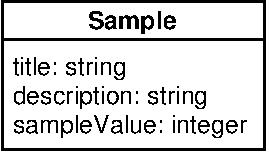
\includegraphics[scale = 0.7]{sampleschema}%
\lthtmlpictureZ
\lthtmlcheckvsize\clearpage}

{\newpage\clearpage
\lthtmlfigureA{example38}%
\begin{example}
<element1 attributeA="attributeA-value">element1-value</element1>
<element2 attributeB="attributeB-value" attributeC="attributeC-value">
  <element3>element3-value</element3>
  <element4 attributeD="attributeD-value">element4-value</element4>
</element2>
\end{example}%
\lthtmlfigureZ
\lthtmlcheckvsize\clearpage}


\setlength{\tabcolsep}{20 pt}%

\setlength{\tabcolsep}{20 pt}

\setlength{\extrarowheight}{5pt}%

\setlength{\extrarowheight}{5pt}
\stepcounter{section}

\setlength{\tabcolsep}{6 pt}%

\setlength{\tabcolsep}{6 pt}
{\newpage\clearpage
\lthtmlpictureA{tex2html_wrap794}%
\includegraphics[scale = 0.7]{sampleschema-abstract}%
\lthtmlpictureZ
\lthtmlcheckvsize\clearpage}

{\newpage\clearpage
\lthtmlfigureA{example130}%
\begin{example}
<xs:complexType name="Sample" abstract="true">
  ...
</xs:complexType>
\end{example}%
\lthtmlfigureZ
\lthtmlcheckvsize\clearpage}

\stepcounter{subsection}

\setlength{\tabcolsep}{12 pt}%

\setlength{\tabcolsep}{12 pt}

\setlength{\tabcolsep}{5 pt}%

\setlength{\tabcolsep}{5 pt}

\setlength{\tabcolsep}{5 pt}%

\setlength{\tabcolsep}{5 pt}
\stepcounter{subsection}
{\newpage\clearpage
\lthtmlpictureA{tex2html_wrap820}%
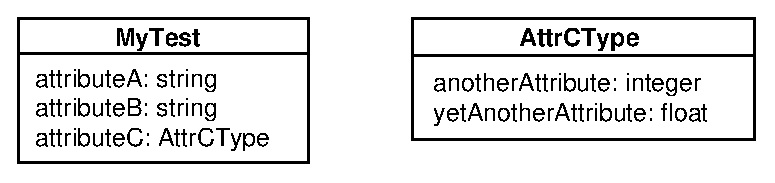
\includegraphics[scale = 0.7]{someschema-uml}%
\lthtmlpictureZ
\lthtmlcheckvsize\clearpage}

{\newpage\clearpage
\lthtmlfigureA{example223}%
\begin{example}
obj.attributeA
obj.attributeB
obj.attributeC.anotherAttribute
obj.attributeC.yetAnotherAttribute
\end{example}%
\lthtmlfigureZ
\lthtmlcheckvsize\clearpage}

{\newpage\clearpage
\lthtmlfigureA{example229}%
\begin{example}
<MyTest attributeA="foo" attributeB="bar">
  <attributeC anotherAttribute="2" yetAnotherAttribute="4.3"/>
</MyTest>
\end{example}%
\lthtmlfigureZ
\lthtmlcheckvsize\clearpage}

{\newpage\clearpage
\lthtmlfigureA{exampleTight236}%
\begin{exampleTight}
<xs:complexType name="AttrCType">
  <xs:attribute name="anotherAttribute" type="xs:integer"/>
  <xs:attribute name="yetAnotherAttribute" type="xs:float"/>
</xs:complexType>
\par <xs:complexType name="MyTest">
  <xs:attribute name="attributeA" type="xs:string"/>
  <xs:attribute name="attributeB" type="xs:string"/>
  <xs:element   name="attributeC" type="AttrCType"/>
</xs:complexType>
\end{exampleTight}%
\lthtmlfigureZ
\lthtmlcheckvsize\clearpage}

\stepcounter{subsection}
\stepcounter{subsubsection}
{\newpage\clearpage
\lthtmlpictureA{tex2html_wrap846}%
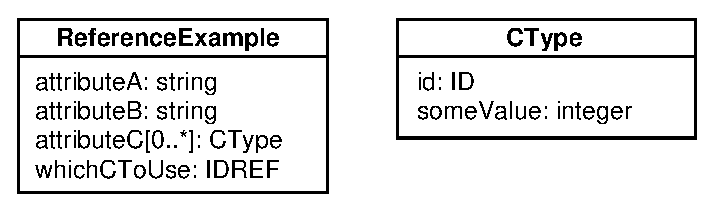
\includegraphics[scale = 0.7]{id-example}%
\lthtmlpictureZ
\lthtmlcheckvsize\clearpage}

{\newpage\clearpage
\lthtmlfigureA{example264}%
\begin{example}
<xs:complexType name="CType">
  <xs:attribute name="id"        type="xs:ID"/>
  <xs:attribute name="someValue" type="xs:integer"/>
</xs:complexType>
\par <xs:complexType name="ReferenceExample">
  <xs:attribute name="attributeA" type="xs:string"/>
  <xs:attribute name="attributeB" type="xs:string"/>
  <xs:element   name="listOfAttributeCs">
    <xs:complexType>
      <xs:element name="attributeC" type="CType" minOccurs="0" maxOccurs="unbounded"/>
    </xs:complexType>
  </xs:element>
  <xs:attribute name="whichCToUse" type="xs:IDREF"/>
</xs:complexType>
\end{example}%
\lthtmlfigureZ
\lthtmlcheckvsize\clearpage}

{\newpage\clearpage
\lthtmlfigureA{example266}%
\begin{example}
<ReferenceExample attributeA="something" attributeB="something else" whichCToUse="c2">
  <listOfAttributeCs> 
    <attributeC id="c1" someValue="42"/>
    <attributeC id="c2" someValue="24"/>
    <attributeC id="c3" someValue="99"/>
  </listOfAttributeCs>
</ReferenceExample>
\end{example}%
\lthtmlfigureZ
\lthtmlcheckvsize\clearpage}

\stepcounter{subsubsection}
{\newpage\clearpage
\lthtmlpictureA{tex2html_wrap860}%
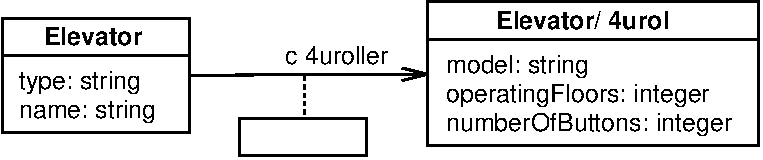
\includegraphics[scale = 0.7]{two-classes}%
\lthtmlpictureZ
\lthtmlcheckvsize\clearpage}


\setlength{\tabcolsep}{20 pt}%

\setlength{\tabcolsep}{20 pt}
{\newpage\clearpage
\lthtmlfigureA{example336}%
\begin{example}
<xs:complexType name="XLink">
  <xs:attribute name="xlink:type" type="string" use="default" value="simple"/>
  <xs:attribute name="xlink:href" type="xs:uriReference"/>
</xs:complexType>
\par <xs:complexType name="Elevator">
  <xs:attribute name="type" type="xs:string"/>
  <xs:attribute name="name" type="xs:string"/>
  <xs:element   name="controller" type="XLink"/>
</xs:complexType>
\end{example}%
\lthtmlfigureZ
\lthtmlcheckvsize\clearpage}

{\newpage\clearpage
\lthtmlfigureA{example338}%
\begin{example}
<Elevator type="Argo K21" name="Main">
  <controller xlink:href="http://www.myserver.net/db/controllers/kc9"/> 
</Elevator>
\end{example}%
\lthtmlfigureZ
\lthtmlcheckvsize\clearpage}

\stepcounter{subsection}
{\newpage\clearpage
\lthtmlpictureA{tex2html_wrap884}%

\includegraphics[scale = 0.7]{xinclude}%
\lthtmlpictureZ
\lthtmlcheckvsize\clearpage}

{\newpage\clearpage
\lthtmlfigureA{example348}%
\begin{example}
<xs:complexType name="XInclude">
  <xs:attribute name="xinclude:href" type="xs:uriReference"/>
</xs:complexType>
\par <xs:complexType name="Bottle">
  <xs:attribute name="capacity"       type="xs:float"/>
  <xs:attribute name="capacity_units" type="xs:string"/>
  <xs:element   name="brand"          type="XInclude"/>
</xs:complexType>
\end{example}%
\lthtmlfigureZ
\lthtmlcheckvsize\clearpage}

{\newpage\clearpage
\lthtmlfigureA{example350}%
\begin{example}
<Bottle capacity="5.0" capacity_units="gallon">
  <brand xinclude:href="http://www.myserver.net/bottledb/maker52"/> 
</Bottle>
\end{example}%
\lthtmlfigureZ
\lthtmlcheckvsize\clearpage}

\stepcounter{subsection}
{\newpage\clearpage
\lthtmlfigureA{wrapfigure354}%
\begin{wrapfigure}{r}{2.2in}
  \begin{center}
    \begin{tabular}{rl}
      1 & exactly one\\
      0,1 & zero or one\\
      0..4 & between zero and four\\
      3,7 & either three or seven\\
      0..* & zero or more\\
      \textrm{*} & zero or more\\
      1..* & one or more
    \end{tabular}
  \end{center}
\end{wrapfigure}%
\lthtmlfigureZ
\lthtmlcheckvsize\clearpage}

\stepcounter{subsubsection}

\setlength{\tabcolsep}{20 pt}%

\setlength{\tabcolsep}{20 pt}
{\newpage\clearpage
\lthtmlpictureA{tex2html_wrap906}%
\includegraphics[scale = 0.7]{simple-attr-list}%
\lthtmlpictureZ
\lthtmlcheckvsize\clearpage}

{\newpage\clearpage
\lthtmlfigureA{example392}%
\begin{example}
<xs:complexType name="SomeThing">
  <xs:attribute name="attributeA" type="xs:string"/>
  <xs:element   name="listOfAttributeBs">
    <xs:complexType>
      <xs:element name="attributeB" type="xs:string"
                  minOccurs="0" maxOccurs="unbounded"/>
    </xs:complexType>
  </xs:element>
</xs:complexType>
\end{example}%
\lthtmlfigureZ
\lthtmlcheckvsize\clearpage}

{\newpage\clearpage
\lthtmlfigureA{example401}%
\begin{example}
<SomeThing attributeA="123">
  <listOfAttributeBs>
    <attributeB value="first string"/>
    <attributeB value="second string"/>
    <attributeB value="third string"/>
  </listOfAttributeBs>
</SomeThing>
\end{example}%
\lthtmlfigureZ
\lthtmlcheckvsize\clearpage}

\stepcounter{subsubsection}

\setlength{\tabcolsep}{20 pt}%

\setlength{\tabcolsep}{20 pt}
{\newpage\clearpage
\lthtmlpictureA{tex2html_wrap918}%
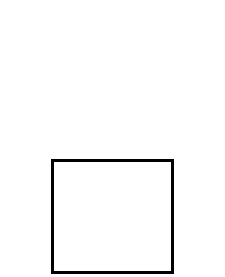
\includegraphics[scale = 0.7]{complex-attr-list}%
\lthtmlpictureZ
\lthtmlcheckvsize\clearpage}

{\newpage\clearpage
\lthtmlfigureA{example419}%
\begin{example}
<xs:complexType name="Point">
  <xs:attribute name="x" type="xs:float"/>
  <xs:attribute name="y" type="xs:float"/>
</xs:complexType>
\par <xs:complexType name="Triangle">
  <xs:attribute name="name" type="xs:string"/>
  <xs:element   name="listOfPoints">
    <xs:complexType>
      <xs:element name="point" type="Point"
                  minOccurs="0" maxOccurs="unbounded"/>
    </xs:complexType>
  </xs:element>
</xs:complexType>
\end{example}%
\lthtmlfigureZ
\lthtmlcheckvsize\clearpage}

{\newpage\clearpage
\lthtmlfigureA{example426}%
\begin{example}
<Triangle name="t1">
  <listOfPoints>
    <point x="2.2" y="1.4"/>
    <point x="0.1" y="4.0"/>
    <point x="0.1" y="1.4"/>
  </listOfPoints>
</Triangle>
\end{example}%
\lthtmlfigureZ
\lthtmlcheckvsize\clearpage}

\stepcounter{subsubsection}
{\newpage\clearpage
\lthtmlpictureA{tex2html_wrap928}%
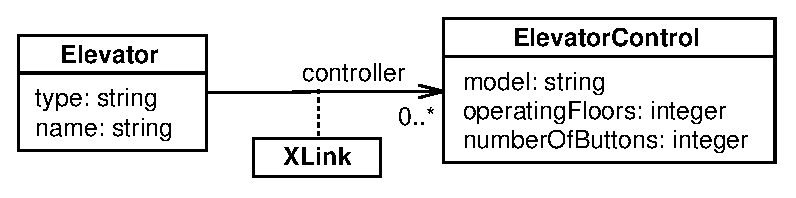
\includegraphics[scale = 0.7]{two-classes-multi}%
\lthtmlpictureZ
\lthtmlcheckvsize\clearpage}

{\newpage\clearpage
\lthtmlpictureA{tex2html_wrap934}%
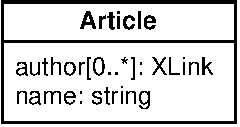
\includegraphics[scale = 0.7]{link-attr-list}%
\lthtmlpictureZ
\lthtmlcheckvsize\clearpage}

{\newpage\clearpage
\lthtmlfigureA{example453}%
\begin{example}
<xs:complexType name="Article">
  <xs:attribute name="name" type="xs:string"/>
  <xs:element   name="listOfAuthors">
    <xs:complexType>
      <xs:element name="author" type="XLink"
                  minOccurs="0" maxOccurs="unbounded"/>
    </xs:complexType>
  </xs:element>
</xs:complexType>
\end{example}%
\lthtmlfigureZ
\lthtmlcheckvsize\clearpage}

{\newpage\clearpage
\lthtmlfigureA{example460}%
\begin{example}
<Article name="t1">
  <listOfAuthors>
    <author xlink:href="http://www.myserver.net/db/author24"/>
    <author xlink:href="http://www.myserver.net/db/author54"/>
  </listOfPoints>
</Article>
\end{example}%
\lthtmlfigureZ
\lthtmlcheckvsize\clearpage}

\stepcounter{subsection}
{\newpage\clearpage
\lthtmlfigureA{example465}%
\begin{example}
<ContainerExample title="This is a title">
  <bigValue>
    This is some long value, something really long, like a big block
    of text that might be too awkward to put inside an attribute value.
  </bigValue>
</ContainerExample>
\end{example}%
\lthtmlfigureZ
\lthtmlcheckvsize\clearpage}


\setlength{\tabcolsep}{10 pt}%

\setlength{\tabcolsep}{10 pt}
{\newpage\clearpage
\lthtmlpictureA{tex2html_wrap948}%
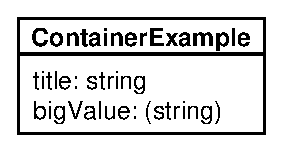
\includegraphics[scale = 0.7]{attribute-container}%
\lthtmlpictureZ
\lthtmlcheckvsize\clearpage}

{\newpage\clearpage
\lthtmlfigureA{example486}%
\begin{example}
<xs:complexType name="ContainerExample">
  <xs:attribute name="title" type="xs:string"/>
  <xs:element   name="bigValue" type="xs:string"/>
</xs:complexType>
\end{example}%
\lthtmlfigureZ
\lthtmlcheckvsize\clearpage}


\setlength{\tabcolsep}{10 pt}%

\setlength{\tabcolsep}{10 pt}
{\newpage\clearpage
\lthtmlpictureA{tex2html_wrap956}%
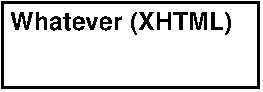
\includegraphics[scale = 0.7]{class-container}%
\lthtmlpictureZ
\lthtmlcheckvsize\clearpage}

{\newpage\clearpage
\lthtmlfigureA{example509}%
\begin{example}
<xs:complexType name="Whatever" content="textOnly">
  <xs:attribute name="bigDeal" type="xs:string"/>
  <xs:attribute name="type" use="fixed" value="XHTML"/>
</xs:complexType>
\end{example}%
\lthtmlfigureZ
\lthtmlcheckvsize\clearpage}

{\newpage\clearpage
\lthtmlfigureA{example516}%
\begin{example}
<Whatever bigDeal="This is an attribute">
  This has a value, but no subelements.
</Whatever>
\end{example}%
\lthtmlfigureZ
\lthtmlcheckvsize\clearpage}

\stepcounter{subsection}

\setlength{\tabcolsep}{20 pt}%

\setlength{\tabcolsep}{20 pt}
{\newpage\clearpage
\lthtmlpictureA{tex2html_wrap972}%

\includegraphics[scale = 0.7]{someschema-constraints}%
\lthtmlpictureZ
\lthtmlcheckvsize\clearpage}

{\newpage\clearpage
\lthtmlpictureA{tex2html_wrap974}%
\includegraphics[scale = 0.7]{someschema-constraints-boxed}%
\lthtmlpictureZ
\lthtmlcheckvsize\clearpage}

{\newpage\clearpage
\lthtmlfigureA{example557}%
\begin{example}
<xs:complexType name="AnExample">
  <xs:attribute name="attrA" type="xs:integer"/>
  <xs:attribute name="attrB">
    <xs:simpleType base="xs:string">
      <xs:enumeration value="val1"/>
      <xs:enumeration value="val2"/>
      <xs:enumeration value="val3"/>
    </xs:simpleType>
  </xs:attribute>
</xs:complexType>
\end{example}%
\lthtmlfigureZ
\lthtmlcheckvsize\clearpage}

{\newpage\clearpage
\lthtmlpictureA{tex2html_wrap982}%
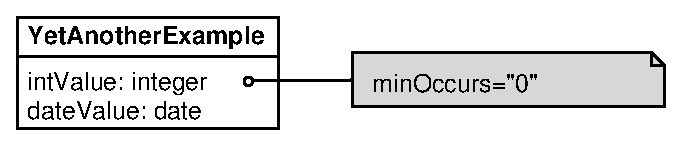
\includegraphics[scale = 0.7]{minoccurs}%
\lthtmlpictureZ
\lthtmlcheckvsize\clearpage}

{\newpage\clearpage
\lthtmlfigureA{example566}%
\begin{example}
<xs:complexType name="YetAnotherExample">
  <xs:attribute name="intValue"  type="xs:integer" minOccurs="0"/>
  <xs:attribute name="dateValue" type="xs:date"/>
</xs:complexType>
\end{example}%
\lthtmlfigureZ
\lthtmlcheckvsize\clearpage}

{\newpage\clearpage
\lthtmlpictureA{tex2html_wrap988}%
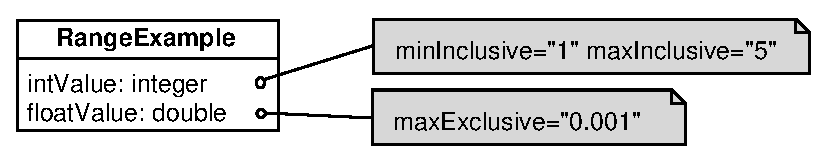
\includegraphics[scale = 0.7]{min-max}%
\lthtmlpictureZ
\lthtmlcheckvsize\clearpage}

{\newpage\clearpage
\lthtmlfigureA{example579}%
\begin{example}
<xs:complexType name="RangeExample">
  <xs:attribute name="intValue"   type="xs:integer" minInclusive="1" maxInclusive="10"/>
  <xs:attribute name="floatValue" type="xs:double"  maxExclusive="0.001"/>
</xs:complexType>
\end{example}%
\lthtmlfigureZ
\lthtmlcheckvsize\clearpage}

\stepcounter{subsection}

\setlength{\tabcolsep}{20 pt}%

\setlength{\tabcolsep}{20 pt}
{\newpage\clearpage
\lthtmlpictureA{tex2html_wrap1006}%
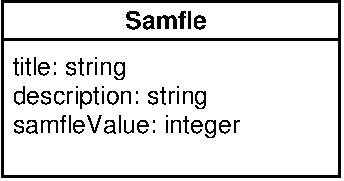
\includegraphics[scale = 0.7]{sampleschema-units}%
\lthtmlpictureZ
\lthtmlcheckvsize\clearpage}

{\newpage\clearpage
\lthtmlfigureA{example606}%
\begin{example}
<xs:simpleType name="Units" base="xs:string">
  <xs:enumeration value="m"/>
  <xs:enumeration value="cm"/>
  <xs:enumeration value="mm"/>
\par <!-- and so on ... -->
\par </xs:simpleType>
\end{example}%
\lthtmlfigureZ
\lthtmlcheckvsize\clearpage}

\stepcounter{subsection}

\setlength{\tabcolsep}{30 pt}%

\setlength{\tabcolsep}{30 pt}
{\newpage\clearpage
\lthtmlpictureA{tex2html_wrap1026}%
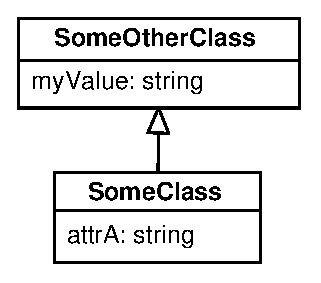
\includegraphics[scale = 0.7]{someschema-inherit}%
\lthtmlpictureZ
\lthtmlcheckvsize\clearpage}

{\newpage\clearpage
\lthtmlfigureA{example652}%
\begin{example}
<xs:complexType name="SomeOtherClass">
  <xs:attribute name="myValue" type="xs:string"/>
</xs:complexType>
\par <xs:complexType name="SomeClass" base="SomeOtherClass" derivedBy="extension">
  <xs:attribute name="attrA" type="xs:string"/>
</xs:complexType>
\end{example}%
\lthtmlfigureZ
\lthtmlcheckvsize\clearpage}

\stepcounter{section}
\stepcounter{section}
\setcounter{secnumdepth}{-1}
\appendix
\stepcounter{section}

\setlength{\parskip}{1.2ex}%

\setlength{\parskip}{1.2ex}

\end{document}
